\documentclass[%
12pt, %
final, % 
oneside, % 
onecolumn, %  
centertags]{article} % относится к классу article и размер шрифта 12 пунктовб, {article: статья, report: отчеты и диссертации, book: книга, letter: письмо}

% \usepackage{fontspec}
 
% \setmainfont{Times New Roman}

% \documentclass[a4paper, 12pt]{report}

\topmargin= -30pt % насколько сверху будет страница
\textheight= 650pt


\usepackage[utf8]{inputenc} % задает кодировку, utf-8 кодировка, включающая в себя знаки почти всех языков мира
\usepackage[english]{babel} % подключает необходимые языки, основным языком является английский

\selectlanguage{english} % настройки будут на английском, но писать будет на русском

\usepackage{euscript}
\usepackage{supertabular}

\renewcommand{\baselinestretch}{1.0} 

\usepackage[colorlinks=true,linkcolor=blue,unicode=true,urlcolor = blue]{hyperref} %hypered
\usepackage[pdftex]{graphicx} % для графики

\usepackage{amsthm, amssymb, amsmath, amsfonts} % математический пакет, математические шрифты
\usepackage{textcomp}
\usepackage[noend]{algorithmic}
\usepackage[ruled]{algorithm}
\usepackage{lipsum}
\usepackage{indentfirst}
\usepackage{babel}
\usepackage{pgfplots}
\usepackage{setspace}
\usepackage{xcolor}
\usepackage{hyperref}
\usepackage{subfigure}

\setcounter{secnumdepth}{5}
\setcounter{tocdepth}{5}
\newcommand\simpleparagraph[1]{%
  \stepcounter{paragraph}\paragraph*{\theparagraph\quad{}#1}}
\usepackage{listings}
% \usepackage{xcolor}
%\usepackage{minted}

\lstset { %
     language=C++,
     backgroundcolor=\color{black!5}, % set backgroundcolor
     basicstyle=\footnotesize,% basic font setting
}


\linespread{1.0} 
\setlength{\parindent}{2.4em}
\setlength{\parskip}{0.1em}

\pgfplotsset{compat=1.9}
\pgfplotsset{model/.style = {blue, samples = 100}} 
\pgfplotsset{experiment/.style = {red}}

\theoremstyle{plain}
\binoppenalty=10000

\newtheorem{theorem}{Theorem}[section] % theorem

\theoremstyle{definition}
% \newtheorem{definition}{Определение}[subsection]
\newtheorem{definition}{Definition}[subsection]

\theoremstyle{remark}
% \newtheorem{remark}{Замечание}[section]

% \newtheorem{corollary}{Следствие}

% \newtheorem{proposition}{Proposition}

% \newtheorem{example}{Пример}

% \newtheorem{lemma}{Лемма}[section]

\renewcommand*{\proofname}{Proof}

\graphicspath{ {./images/} }


% \usepackage{amsmath,amsfonts,amssymb, setspace}  % Разнообразные математические команды и значки
% \usepackage{indentfirst}     % Отступ в первом абзаце

% \pagestyle{empty}
\usepackage[left=2.5cm, right=1.5cm, top=2.5cm, bottom=2.5cm]{geometry}
\usepackage[medium]{titlesec}
\usepackage{graphicx}
% \graphicspath{ {./images/} }

\begin{document}

	\begin{titlepage} 
		\begin{center}
		\textbf{}\\[2.0cm]
		\LARGE FEDERAL STATE AUTONOMOUS EDUCATIONAL INSTITUTION OF HIGHER EDUCATION \\[0.5cm]
		\Large ITMO UNIVERSITY \\[3cm]
		\LARGE Report\\
		\Large MPI. Assignments $20-21$ \\
		\Large Parallel algorithms for the analysis and synthesis of data \\[4cm]


		\begin{flushright}
		Performed by\\
		Aleksandr Shirokov\\
		J4133c\\
		Accepted by\\
		Petr Andriushchenko

		Deadline: 26.12.21
		\end{flushright}

		\vfill 

		{\Large {St. Petersburg}} \par
		{\Large {2021}}
		\end{center} 
	\end{titlepage}

\tableofcontents
\newpage


\section{Assignments}

\subsection{Assignment 20. MPI. Parallel I \/ O. Working with files. Access to data. Buffered reading from a file}

\subsubsection{Formulation of the problem}

Understand the new functions in \textsc{Assignment20.c}, complete the program according to the 
assignment, explain the execution of the program.

Write a function that will create a file \textbf{"file.txt"} with random content (or with specific text). The 
function must be executed before the program reads the contents of the file. Run the program 
on one process. Check if the contents of the file are displayed correctly. Add an option that will 
delete the file on close

\subsubsection{Example of launch parameters and output. Detailed description of solution}

Code for \textbf{assignment 20} is \href{https:\//github.com/aptmess/parallel_algorithms/blob/master/HT/hw_mpi/Assignment20.c}{here}.

Compilation example: \textsc{mpic++ -o ./cpf/20.o Assignment20.c}

Launch example: 

\begin{itemize}
	\item \textsc{mpirun --oversubscribe -np 1 ./cpf/20.o} - without delete option
	\begin{center}
	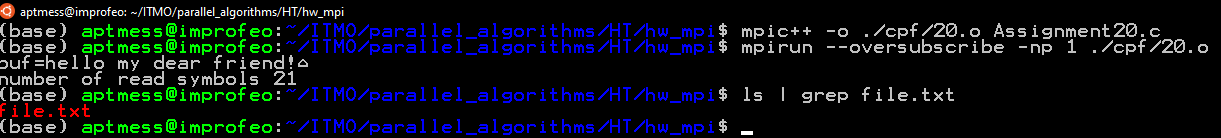
\includegraphics[scale=0.5]{20.no.option.png}

	File exists and also their is input
	\end{center}
	\item \textsc{mpirun --oversubscribe -np 1 ./cpf/20.o --delete-file} - with delete option
	\begin{center}
	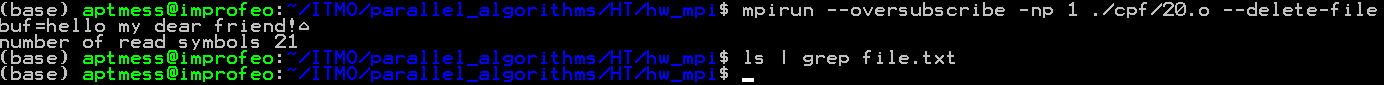
\includegraphics[scale=0.45]{20.yes.option.png}

	As we can see the file is deleted.
	\end{center}

\end{itemize}


Let's move to the the code and explain how it works.

\begin{center}
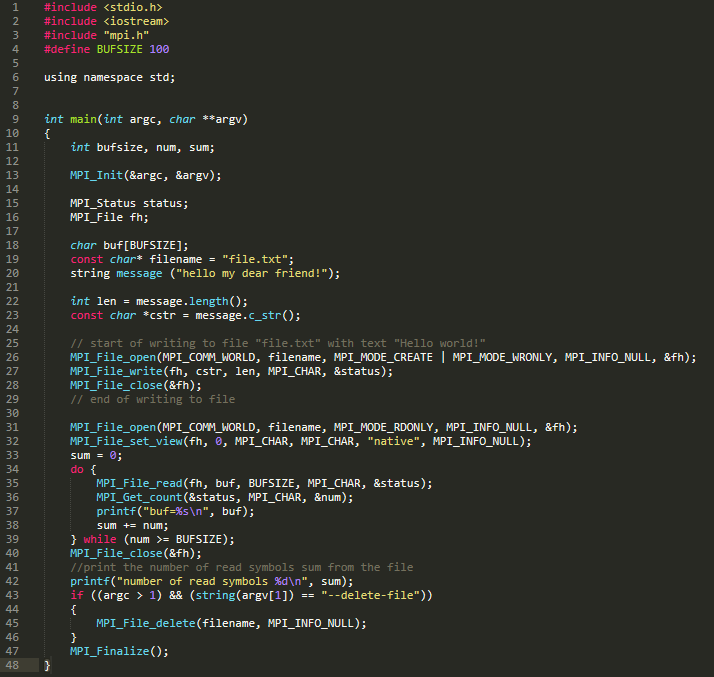
\includegraphics[scale=0.9]{20.png}

Assignment20 code
\end{center}

In this lab there are new functions of MPI that works with some I\/O (input and output) operations with files. In lines $19-20$ there is a filename and string which will be filled in file, in line $25-29$ there is a function that open files (\textsc{MPI\_File\_open}), write in file message (\textsc{MPI\_File\_write}) and standard closing \textsc{MPI\_File\_Close}. After that weopen file and read only mode, \textsc{MPI\_File\_set\_view} function changes process’s view of data in file (collective) and in lines $34-39$ while end on the file count the amount of symbols in file. File closing in line $40$, printing the number of read sybmols sum from the file and if there is a option \textsc{--delete-file} there is function to delete file. Program works correctly 
for each option of running program as we checking it with grep higher. 

\newpage

\subsection{Assignment 21. MPI. Parallel I \/ O. Working with files. Access to data. Collective reading from a file}

\subsubsection{Formulation of the problem}

Understand the new functions in \textsc{Assignment21.c}, complete the program according 
to the assignment, explain the execution of the program.

Create a file and fill it with bulky text, output the content in parallel. Change the step 
of reading the contents of the file and the number of characters to be output by each 
process.

\subsubsection{Example of launch parameters and output. Detailed description of solution}

Code for \textbf{assignment 21} is \href{https:\//github.com/aptmess/parallel_algorithms/blob/master/HT/hw_mpi/Assignment21.c}{here}.

Compilation example: \textsc{mpic++ -o ./cpf/21.o Assignment21.c}

Launch example: 

\begin{center}
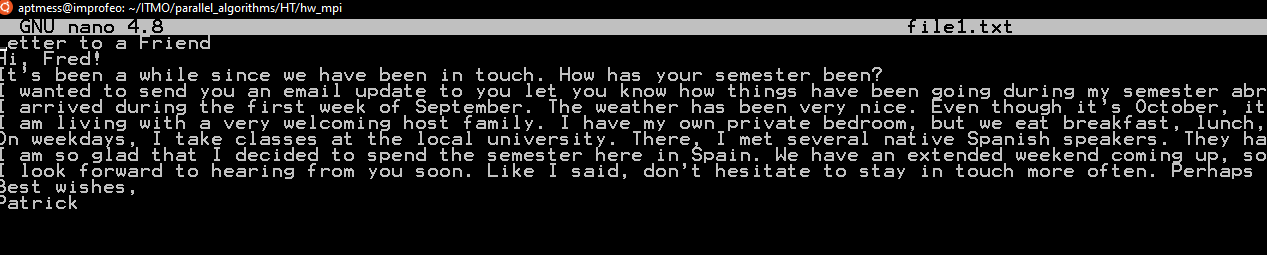
\includegraphics[scale=0.45]{21.content.png}

It is a text in file \textbf{file1.txt}
\end{center}

\begin{center}
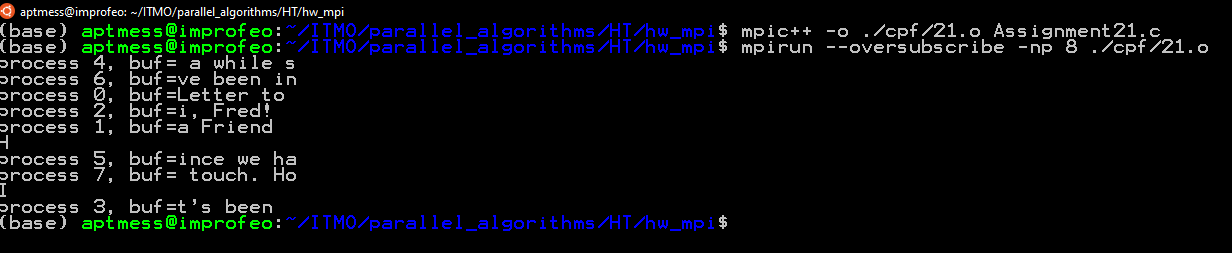
\includegraphics[scale=0.45]{21.run.png}

Run program with $10$ sybmols per process. Let's change amount of sybmols to $30$
\end{center}

\begin{center}
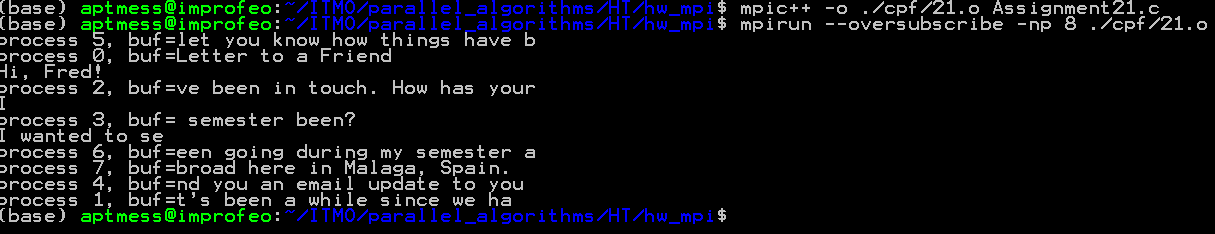
\includegraphics[scale=0.45]{21.run2.png}

Amount of sybmols per process is $30$.
\end{center}

Let's move to the the code and explain how it works.

\begin{center}
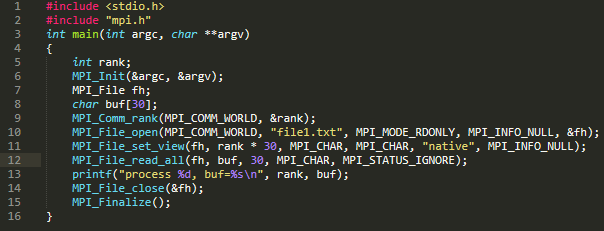
\includegraphics[scale=0.9]{21.code.png}

Assignment21 code
\end{center}

As we can see our program read file \textbf{file1.txt} in parallel mode by fixed amount of sybmols (i have increased amount of sybmols from $10$ to $30$ as it is shown higher) for each process there is a formula which sybmols each process is reading using function \textsc{MPI\_File\_set\_view} - $[\left(20\cdot\operatorname{rank}\right)\ldots \left( 20 \cdot (\operatorname{rank} + 1) - 1 \right)]$. As we can see program works correctly and we can control with parallel mode the velocity of reading files - it is very common operation in MPI i think. That's all!

\subsection{Appendix}


 
The link to the sourse code which is placed on my \href{https://github.com/aptmess/parallel_algorithms}{github}.


\end{document}